\documentclass{beamer}
\setbeamertemplate{footline}[page number]
\date{}
\author{}
\institute{}

%%%%%%% Put these names back in the final version 
%\\Aswathy Rajendra Kurup\\Meenu Ajith}
%\institute{Department of Electrical and Computer Engineering\\The University of New Mexico}
\setbeamercovered{transparent}
\usepackage{setspace}
\usepackage{array}
\usepackage[T1]{fontenc}
\usepackage{graphicx}
\usepackage{amsmath}
\usepackage{amsfonts}
\usepackage{amssymb}
\usepackage{makeidx}
\usefonttheme{serif}
\usepackage{multirow}
\usepackage{booktabs} 
\usepackage{rotating}
\usepackage{color}
\usepackage{float}
\usepackage[latin1]{inputenc}
\usepackage[english]{babel}
\usepackage{amsmath}
\usepackage{amsfonts}
\usepackage{eurosym}
\usepackage{rotating}
\usepackage{multicol}
\usepackage{pythonhighlight}
\usepackage[normalem]{ulem}
\newcommand{\ba}{{\bf a}}
\newcommand{\bb}{{\bf b}}
\newcommand{\bc}{{\bf c}}
\newcommand{\bd}{{\bf d}}
\newcommand{\be}{{\bf e}}
\newcommand{\bbf}{{\bf f}}
\newcommand{\bg}{{\bf g}}
\newcommand{\bh}{{\bf h}}
\newcommand{\bi}{{\bf i}}
\newcommand{\bk}{{\bf k}}
\newcommand{\bl}{{\bf l}}
\newcommand{\bm}{{\bf m}}
\newcommand{\bn}{{\bf n}}
\newcommand{\bo}{{\bf o}}
\newcommand{\bp}{{\bf p}}
\newcommand{\bq}{{\bf q}}
\newcommand{\br}{{\bf r}}
\newcommand{\bs}{{\bf s}}
\newcommand{\bt}{{\bf t}}
\newcommand{\bu}{{\bf u}}
\newcommand{\bv}{{\bf v}}
\newcommand{\bw}{{\bf w}}
\newcommand{\bx}{{\bf x}}
\newcommand{\by}{{\bf y}}
\newcommand{\bz}{{\bf z}}

\newcommand{\bA}{{\bf A}}
\newcommand{\bB}{{\bf B}}
\newcommand{\bC}{{\bf C}}
\newcommand{\bE}{{\bf E}}
\newcommand{\bG}{{\bf G}}
\newcommand{\bH}{{\bf H}}
\newcommand{\bI}{{\bf I}}
\newcommand{\bK}{{\bf K}}
\newcommand{\bL}{{\bf L}}
\newcommand{\bM}{{\bf M}}
\newcommand{\bO}{{\bf O}}
\newcommand{\bQ}{{\bf Q}}
\newcommand{\bR}{{\bf R}}
\newcommand{\bS}{{\bf S}}
\newcommand{\bT}{{\bf T}}
\newcommand{\bV}{{\bf V}}
\newcommand{\bW}{{\bf W}}
\newcommand{\bX}{{\bf X}}
\newcommand{\bY}{{\bf Y}}
\newcommand{\bZ}{{\bf Z}}
\newcommand\uptocnt{\stackrel{\mathclap{\normalfont\mbox{c}}}{\propto}}
\newcommand{\bpt}{{\bf pt}}
\newcommand{\bpl}{{\bf pl}}
\newcommand{\bdp}{{\bf dp}}
\newcommand{\btemp}{{\bf temp}}

\newcommand{\bmu}{{\boldsymbol \mu}}
\newcommand{\bSigma}{{\boldsymbol \Sigma}}
\newcommand{\bsigma}{{\boldsymbol \sigma}}
\newcommand{\bvarPhi}{{\boldsymbol \varPhi}}
\newcommand{\bvarphi}{{\boldsymbol \varphi}}
\newcommand{\bPhi}{{\boldsymbol \Phi}}
\newcommand{\bdelta}{{\boldsymbol \delta}}
\newcommand{\bZero}{{\bf 0}}
\newcommand{\bOne}{{\bf 1}}
\newcommand{\balpha}{{\boldsymbol \alpha}}
\newcommand{\bAlpha}{{\boldsymbol A}}
\newcommand{\btheta}{{\boldsymbol \theta}}

\newcommand{\softmax}{\text{softmax}}
\newcommand{\diag}{\text{diag}}
\newcommand{\sinc}{\mathrm{sinc}}
\newcommand{\argmin}{\mathop{\mathrm{argmin}}}
\newcommand{\infl}{\eta}
\newcommand{\Ind}{\mathrm{I}}
\newcommand{\Real}{\mathbb R}
\newcommand{\Intg}{\mathbb Z}
\newcommand{\Complex}{\mathbb C}
\newcommand{\Natural}{\mathbb N}
\newcommand{\Fourier}[1]{\mathcal{F} \{#1\}}
%\newcommand{\ii}{\mathbbm{i}}
\newcommand{\bphi}{\boldsymbol{\mathit{\phi}}}

\newcommand{\hs}{\hspace{2pt}}
\newcommand{\sign}{\text{sign}}
\author{Manel Mart\'inez-Ram\'on\\Meenu Ajith\\Aswathy Rajendra Kurup}

\usetheme{Madrid}
\usecolortheme{beaver}
\usepackage{tikz}
\usetikzlibrary{fit,arrows,calc,positioning}
\usepackage{listings}
\usepackage{xcolor}
\usepackage{emerald} 
\usepackage[T1]{fontenc} 
\usepackage{verbatim}
\usepackage{graphicx}
\usepackage{epsfig}
\usepackage{psfrag}
\usepackage[english]{babel}
\usepackage{listings}
\usepackage{courier}
\usepackage{color}
 \usepackage{vwcol} 
 \usepackage[english]{babel} % To obtain English text with the blindtext package
\usepackage{blindtext}
\definecolor{codegreen}{rgb}{0,0.6,0}
\definecolor{codegray}{rgb}{0.5,0.5,0.5}
\definecolor{codepurple}{rgb}{0.58,0,0.82}
\definecolor{backcolour}{rgb}{0.95,0.95,0.92}

\lstdefinestyle{mystyle}{
  backgroundcolor=\color{backcolour},   commentstyle=\color{codegreen},
  keywordstyle=\color{magenta},
  numberstyle=\tiny\color{codegray},
  stringstyle=\color{codepurple},
  basicstyle=\ttfamily\footnotesize,
  breakatwhitespace=false,         
  breaklines=true,                 
  captionpos=b,                    
  keepspaces=true,                 
  numbers=left,                    
  numbersep=5pt,                  
  showspaces=false,                
  showstringspaces=false,
  showtabs=false,                  
  tabsize=2
}
\lstset{style=mystyle}

%% Stuff for movies

% %\newcommand{\bt}{{\bf t}}
% \newcommand{\br}{{\bf r}}
% \newcommand{\bs}{{\bf s}}
% \newcommand{\by}{{\bf y}}
% \newcommand{\bz}{{\bf z}}
% \newcommand{\bx}{{\bf x}}
% \newcommand{\bw}{{\bf w}}
% \newcommand{\be}{{\bf e}}
% \newcommand{\bbf}{{\bf f}}
% \newcommand{\bb}{{\bf b}}
% \newcommand{\bd}{{\bf d}}
% \newcommand{\bA}{{\bf A}}
% \newcommand{\bB}{{\bf B}}
% \newcommand{\bL}{{\bf L}}
% \newcommand{\bM}{{\bf M}}

% \newcommand{\bC}{{\bf C}}
% \newcommand{\bI}{{\bf I}}
% \newcommand{\bK}{{\bf K}}
% \newcommand{\bk}{{\bf k}}
% \newcommand{\bT}{{\bf T}}
% \newcommand{\bV}{{\bf V}}
% \newcommand{\bW}{{\bf W}}
% \newcommand{\bX}{{\bf X}}
% \newcommand{\bY}{{\bf Y}}
% \newcommand{\bZ}{{\bf Z}}
% \newcommand{\bm}{{\bf m}}
% \newcommand{\bpt}{{\bf pt}}
% \newcommand{\bpl}{{\bf pl}}
% \newcommand{\bdp}{{\bf dp}}
% \newcommand{\btemp}{{\bf temp}}
% \newcommand{\bl}{{\bf l}}
% \newcommand{\bu}{{\bf u}}
% \newcommand{\bmu}{{\boldsymbol \mu}}
% \newcommand{\bSigma}{{\boldsymbol \Sigma}}
% \newcommand{\bLambda}{{\boldsymbol \Lambda}}

% \newcommand{\bsigma}{{\boldsymbol \sigma}}
% \newcommand{\bvarphi}{{\boldsymbol \varPhi}}
% \newcommand{\btheta}{{\boldsymbol \theta}}
% \newcommand{\bZero}{{\bf 0}}
% \newcommand{\balpha}{{\boldsymbol \alpha}}
% \newcommand{\bpi}{{\boldsymbol \pi}}
% \newcommand{\bxi}{{\boldsymbol \xi}}
% \newcommand{\bdelta}{{\boldsymbol \delta}}
\lstset{
	language=Python,
	basicstyle=\footnotesize\ttfamily\color{black},
	commentstyle = \footnotesize\ttfamily\color{red},
	keywordstyle=\footnotesize\ttfamily\color{blue},
	stringstyle=\footnotesize\ttfamily\color{black},
%	columns=fixed,
%	numbers=left,    
	numberstyle=\tiny,
	stepnumber=1,
	numbersep=5pt,
	tabsize=1,
	extendedchars=true,
	breaklines=true,            
	frame=b,         
	showspaces=false,
	showtabs=true,
	xleftmargin=6pt,
	framexleftmargin=6pt,
	framexrightmargin=2pt,
	framexbottommargin=4pt,
	showstringspaces=false      
}

\lstloadlanguages{
         Python
}

%\graphicspath{ {./images/} }  % Figures path - used in graphicx

%\selectcolormodel{cmyk}

\mode<presentation>

\newcommand{\dred}{darkred!90!black}
\newcommand{\written}{\ECFJD\textcolor{cyan!50!white}}
\newcommand{\hlight}{\textcolor{\dred}}
\newcommand{\Ex}{\textcolor{\dred}{Ex. }}

% remove navigation symbols in full screen mode
\setbeamertemplate{navigation symbols}{}  
\setbeamertemplate{blocks}[rounded][shadow=false]
\setbeamercolor{note page}{fg=black}

\setbeamercolor{title}{fg=\dred}
\setbeamercolor{frametitle}{fg=white}
\setbeamercolor{frametitle}{bg=\dred}
\setbeamercolor{structure}{fg=black,bg=white}
\setbeamercolor{background canvas}{bg=white,fg=black}
\setbeamercolor{normal text}{fg=black,bg=white}
\setbeamercolor{item}{fg=red!80!black,bg=white!}
\addtobeamertemplate{block begin}{\setbeamercolor{block title}{fg=white,bg=\dred}
\setbeamercolor{block body}{fg=white,bg=gray}}{}



\title{4. Convolutional Neural networks}
\subtitle{4.3. Advanced CNN structures}

\addtobeamertemplate{frametitle}{}


\begin{document}
\maketitle


\begin{frame}{Alexnet }
\begin{itemize}
    \item Alex Krizhevsky, Ilya Sutskever and Geoffrey Hinton (2012).
    \item Able to solve the Imagenet image classification problem with 1000 classes. 
    \item Won the 2-12 ImageNet Large Scale Visual Recognition Challenge (LSVRC) conmpetition.
    \item Structure:
    \begin{itemize}
     \item 8 layers and 60M learnable parameters. 
     \item  5 are convolutional layers along with max-pooling layers and 3 fully connected layers and ReLU non-linearity. \item SoftMax with 1000 outputs.
     \end{itemize}
\end{itemize}
\end{frame}
\begin{frame}{Alexnet}
    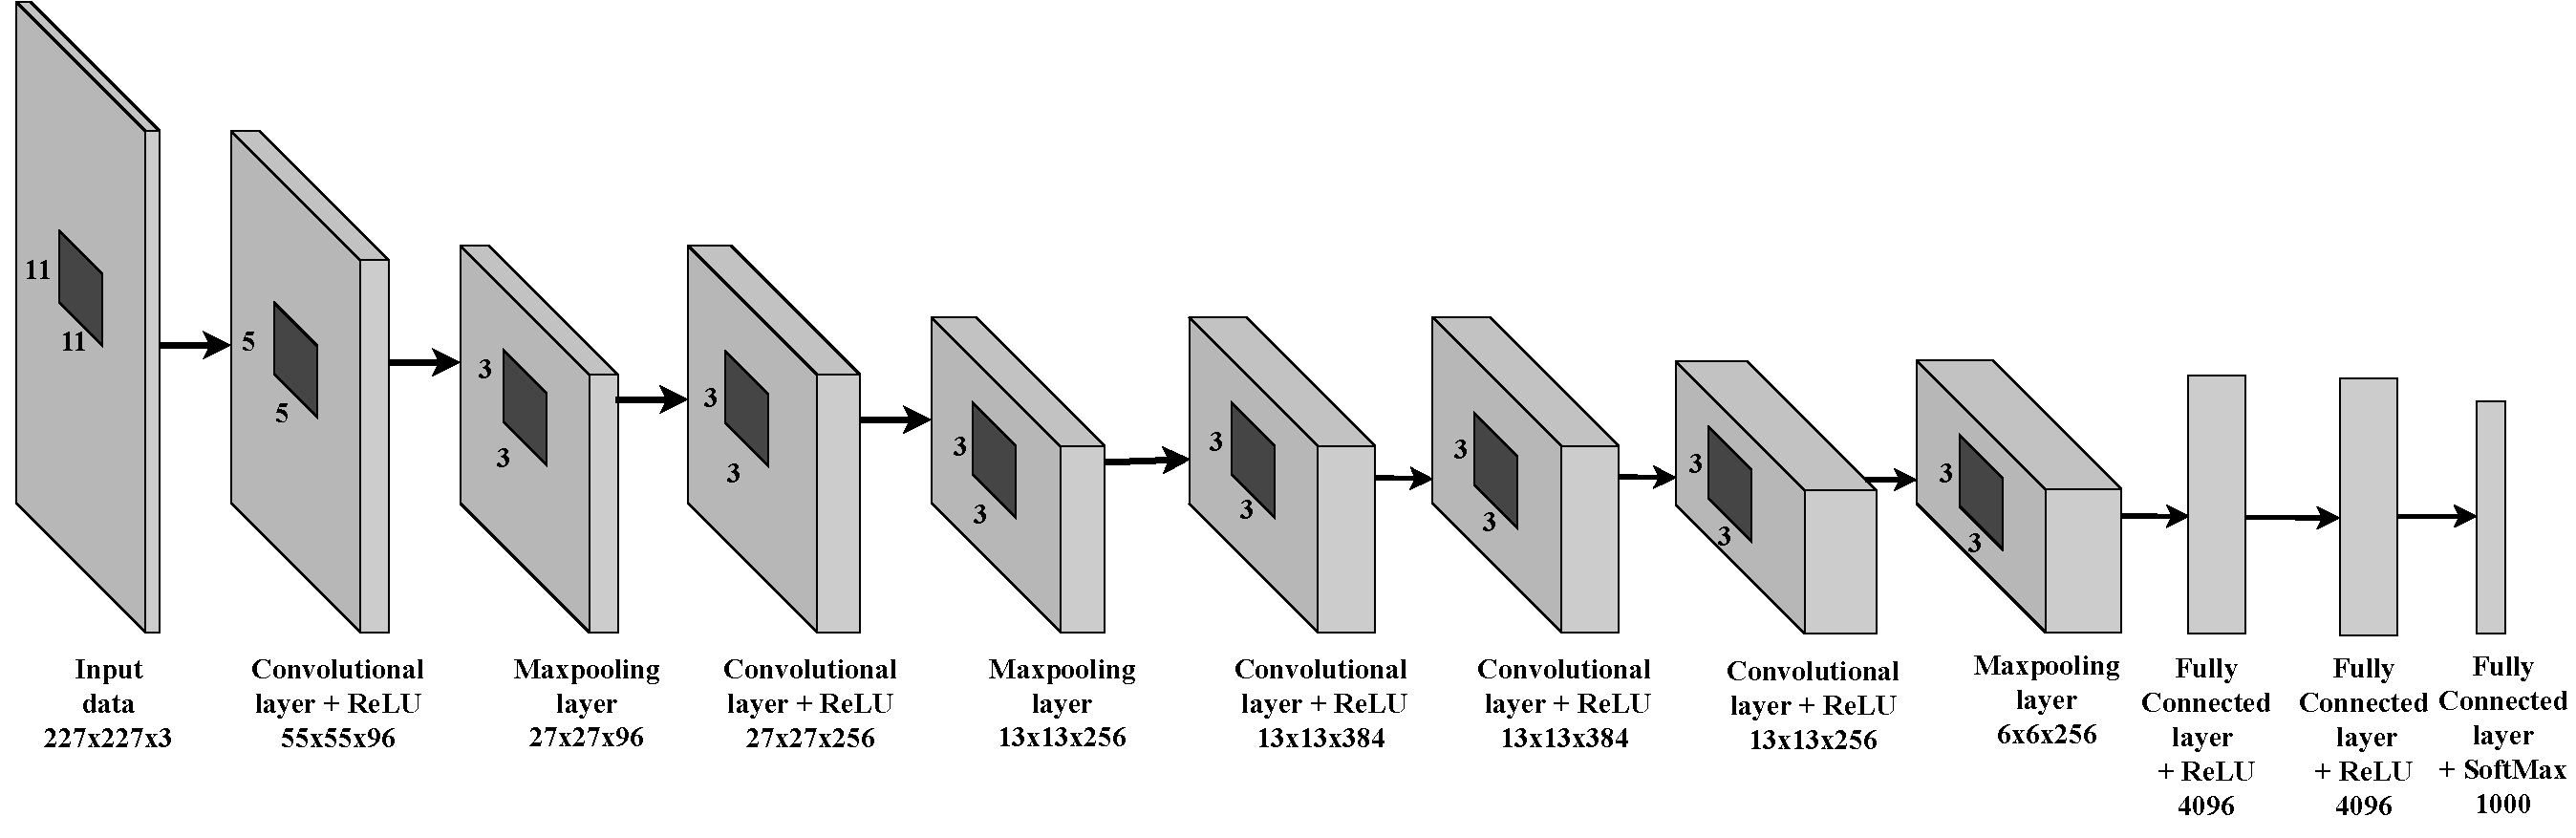
\includegraphics[width=\textwidth]{Module 4 (CNN)/pics/alexnet.pdf}
\end{frame}
\begin{frame}{Alexnet}
\begin{itemize}
    \item RGB images,  $224\times 224 \times 3$ 
    \item The convolutions include a stride of 4 pixels. 
    \item A padding of 3 pixels are possibly used. 
    \item  The fifth convolutional layer contains 256 kernels of size $3\times 3\times 192$ 
    \item Each of the hidden fully connected layers has 4096 neurons. 
    \item Novelties:
    \begin{itemize}
    \item Data augmentation by a factor of 2048 by extracting random patches from the images and altering the intensities of the RGB channels. 
    \item Dropout, ReLU, overlapping pooling, multi-GPU.
    \end{itemize}
\end{itemize}
\end{frame}

\begin{frame}{VGG}

\begin{itemize}
    \item  VGG stands for Visual Geometric Group. This network was developed in the year 2014 by Karen Simonyan and Andrew Zisserman (Oxford University, 2014).
    \item Second place, 2014 ImageNet ILSVRC competition. 
    \item Main idea: increase the depth of the convolutional network in large-scale image recognition settings. 
     \item Smaller convolutional filters were used for increased depth.  
\end{itemize}    
\end{frame}
\begin{frame}{VGG}

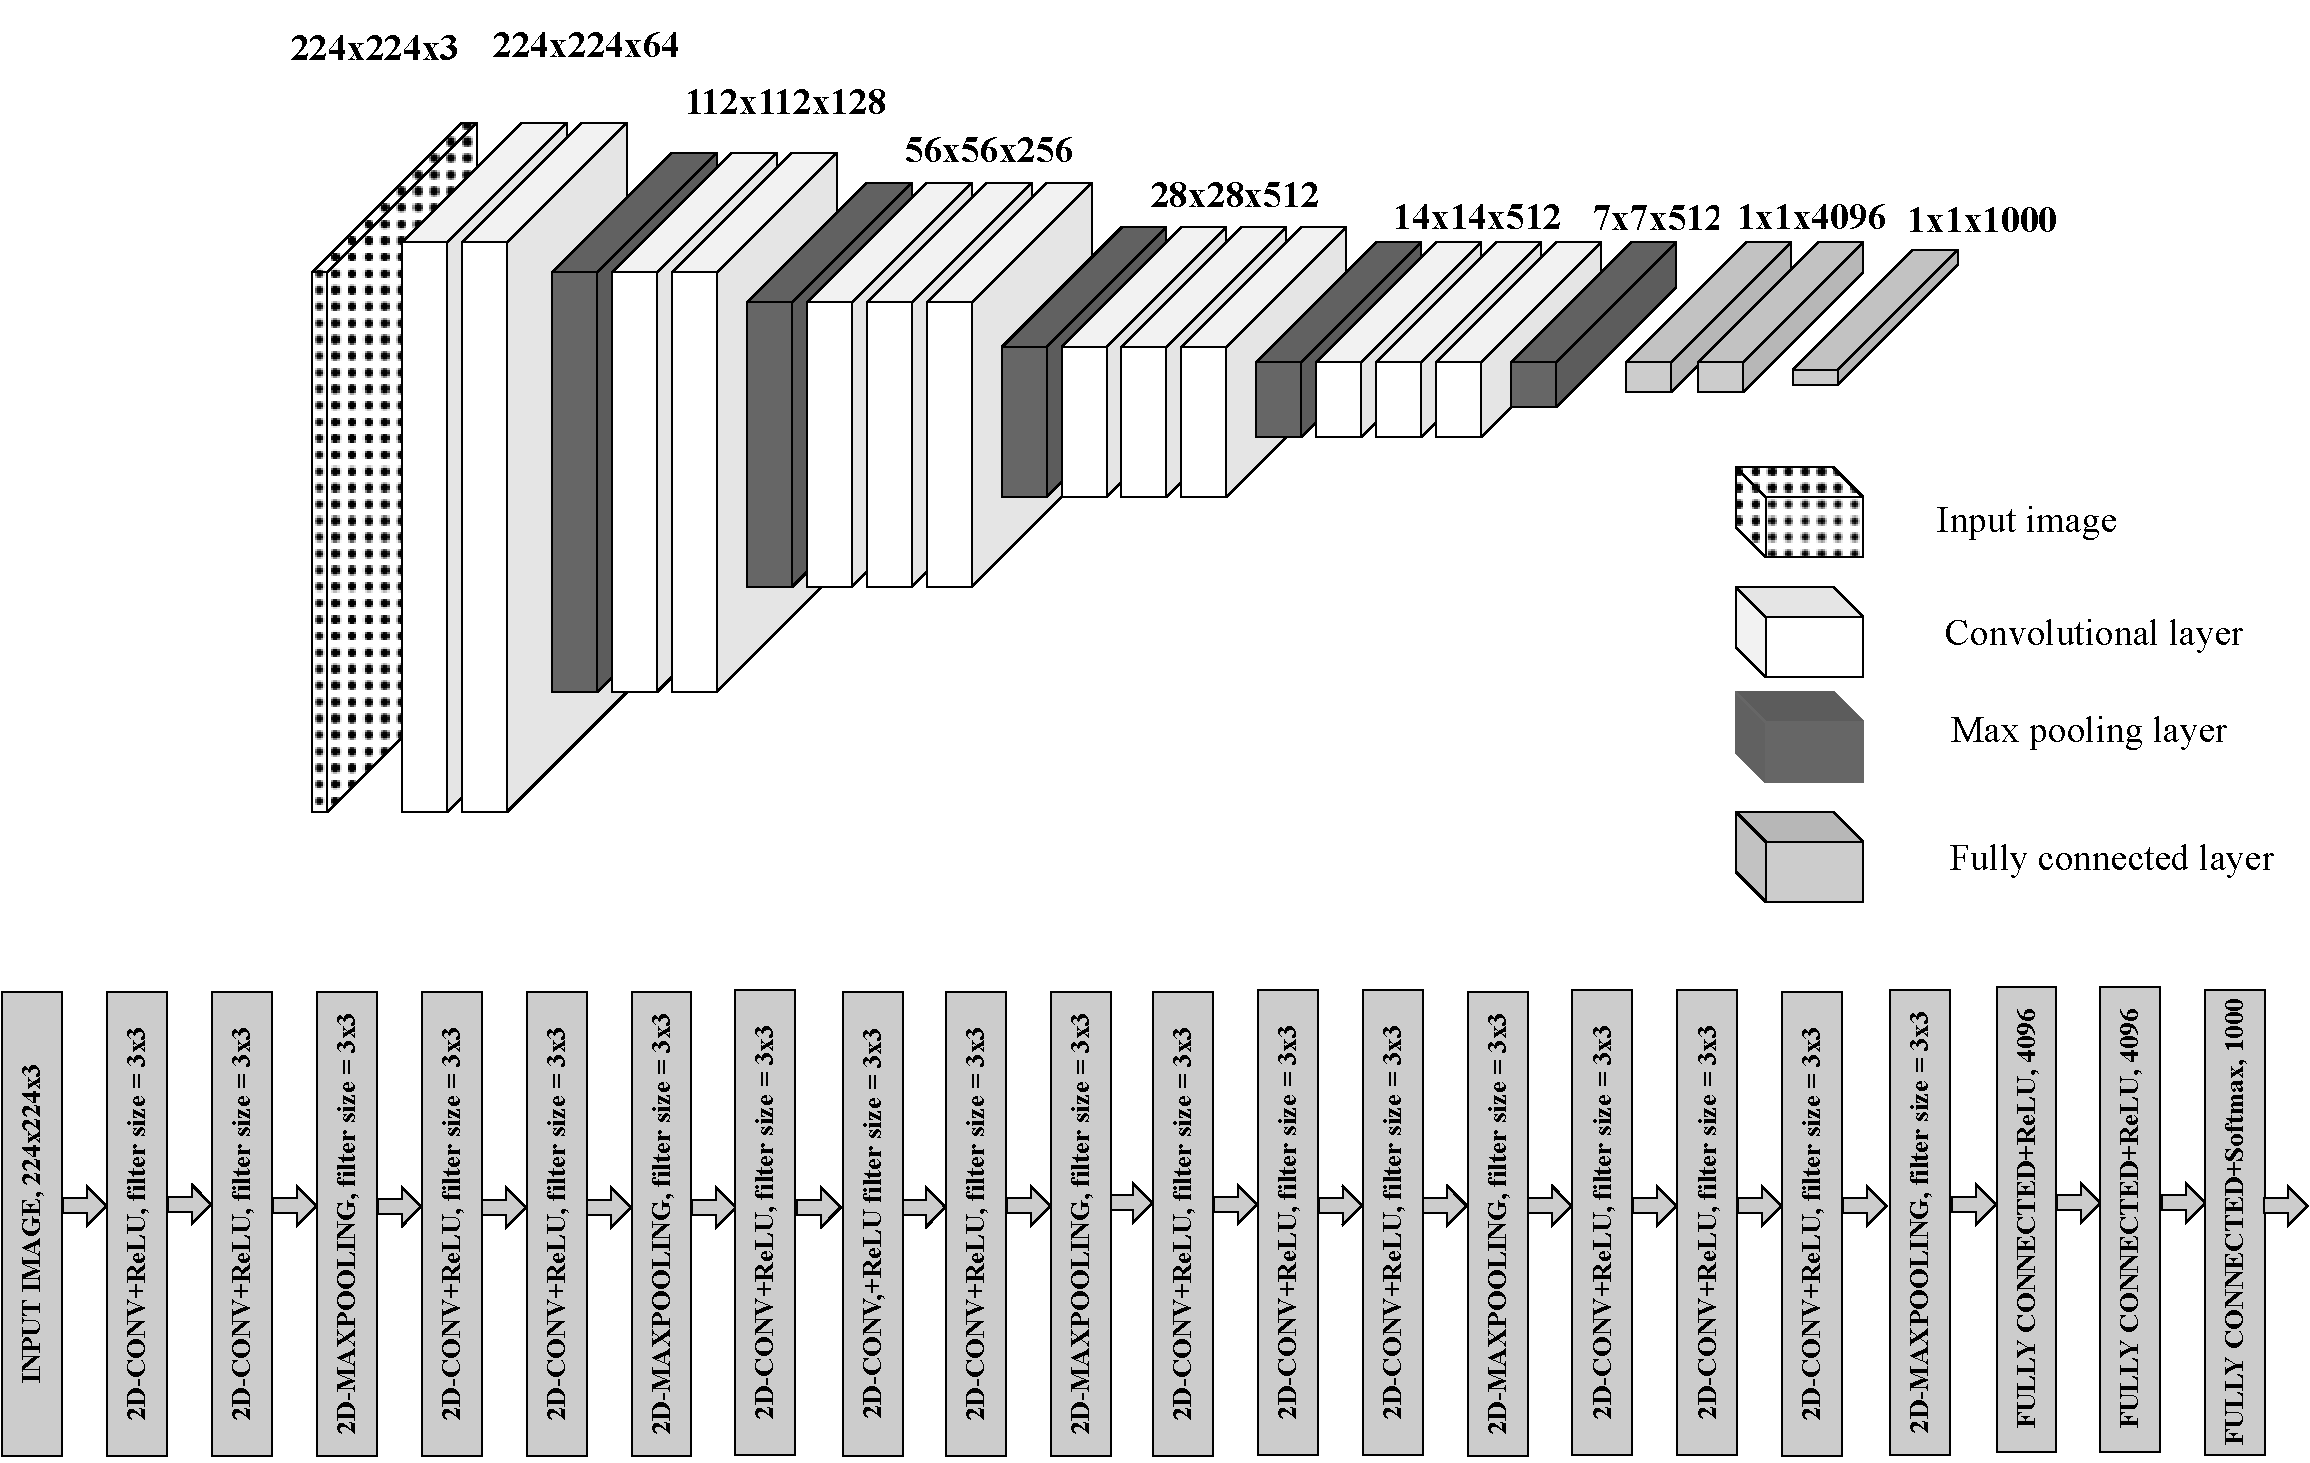
\includegraphics[width=\textwidth]{Module 4 (CNN)/pics/vgg_net.pdf}
    
\end{frame}

\begin{frame}{VGG}
\begin{itemize}
    \item  Depth is achieved through a stack of convolutional layers. 
    \item Convolutional kernels of smaller size ($3\times 3$).
    \item five max-pooling layers with a window size of $2\times2$ and a stride 2. 
    \item ReLU activations. 
    \item Three fully connected layers with 4096, 4096 and 1000 nodes, with softmax activation.
    \item Incorporates 1$\times1$ convolutions, that are just linear transformations. 
\end{itemize}
\end{frame}
\begin{frame}{VGG}
\begin{itemize}
    \item First to use a p[reprocessing block that crops the image to size $224\times224$, extracts the mean RGB value.
    \item Shows that 3$\times$3 kernels stacked several times is as effective as a 5$\times$5 or $7\times7$ kernel. 
    \item 6 versions with 11 layers, 16 layers (VGG16) and 19 layers (VGG19), containing different number of convolution layers, but all of them kept the same number of fully connected layers and nodes.
\end{itemize}
   
\end{frame}

\begin{frame}{Inception}
    \begin{itemize}
        \item Inception-v1/GoogleNet has 22 layers and 5 million parameters. 
        \item Winner of the 2014 ImageNet LSVR Competition. 
        \item Previous structures are focused on increasing the depth. Inception has recurring blocks of convolutional designs called Inception modules. 
        \item Around 100 layers. 
        \item ReLU activations. 
        \item Auxiliary classifiers in order to prevent the vanishing gradient problem.
    \end{itemize}
\end{frame}


\begin{frame}{Inception}

 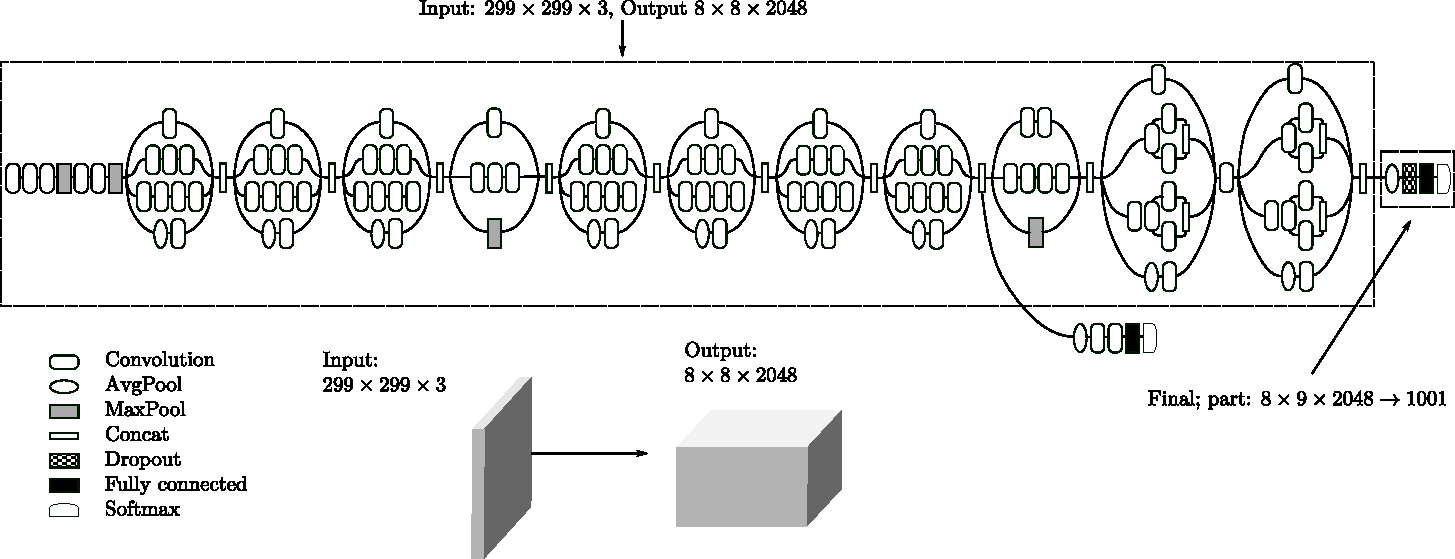
\includegraphics[width=\textwidth]{Module 4 (CNN)/pics/inception-v3.pdf}
    
\end{frame}
\begin{frame}{ResNet}
    \begin{itemize}
        \item Winner of the 2015 ImageNet localization, ImageNet detection, in the LSCR competition and segmentation and detection challenges in the 2015 Common Objects in COntext (COCO) competition.   
    \end{itemize}
\end{frame}

\begin{frame}{ResNet}
        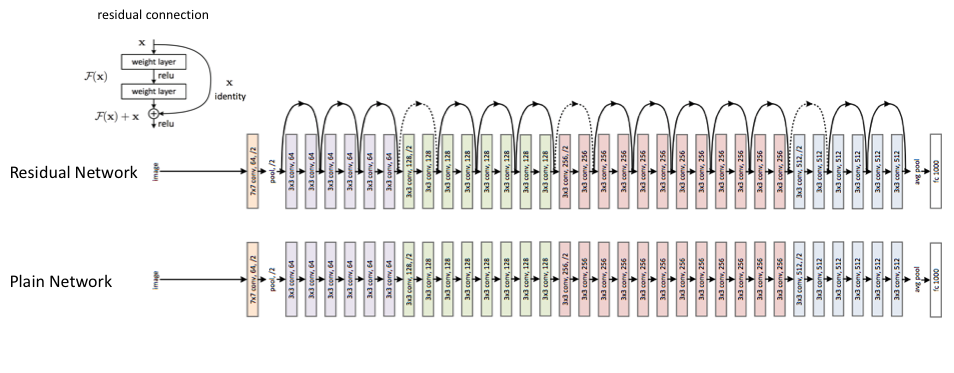
\includegraphics[width=\textwidth]{Module 4 (CNN)/pics/resnet-34.png}
\end{frame}

\begin{frame}{Others}
    \begin{itemize}
    \item Xception, Fran{\c c}ois Chollet (2017).
    \item MobileNet, Google (2017).
    \item Densenet, Cornell University, Tsinghua University, Facebook, 2017.
    \item EfficientNet, Mingxing Tan and Quoc Le (2019).
    
    \end{itemize}
\end{frame}

\begin{frame}{Comparisons}

\begin{center}
    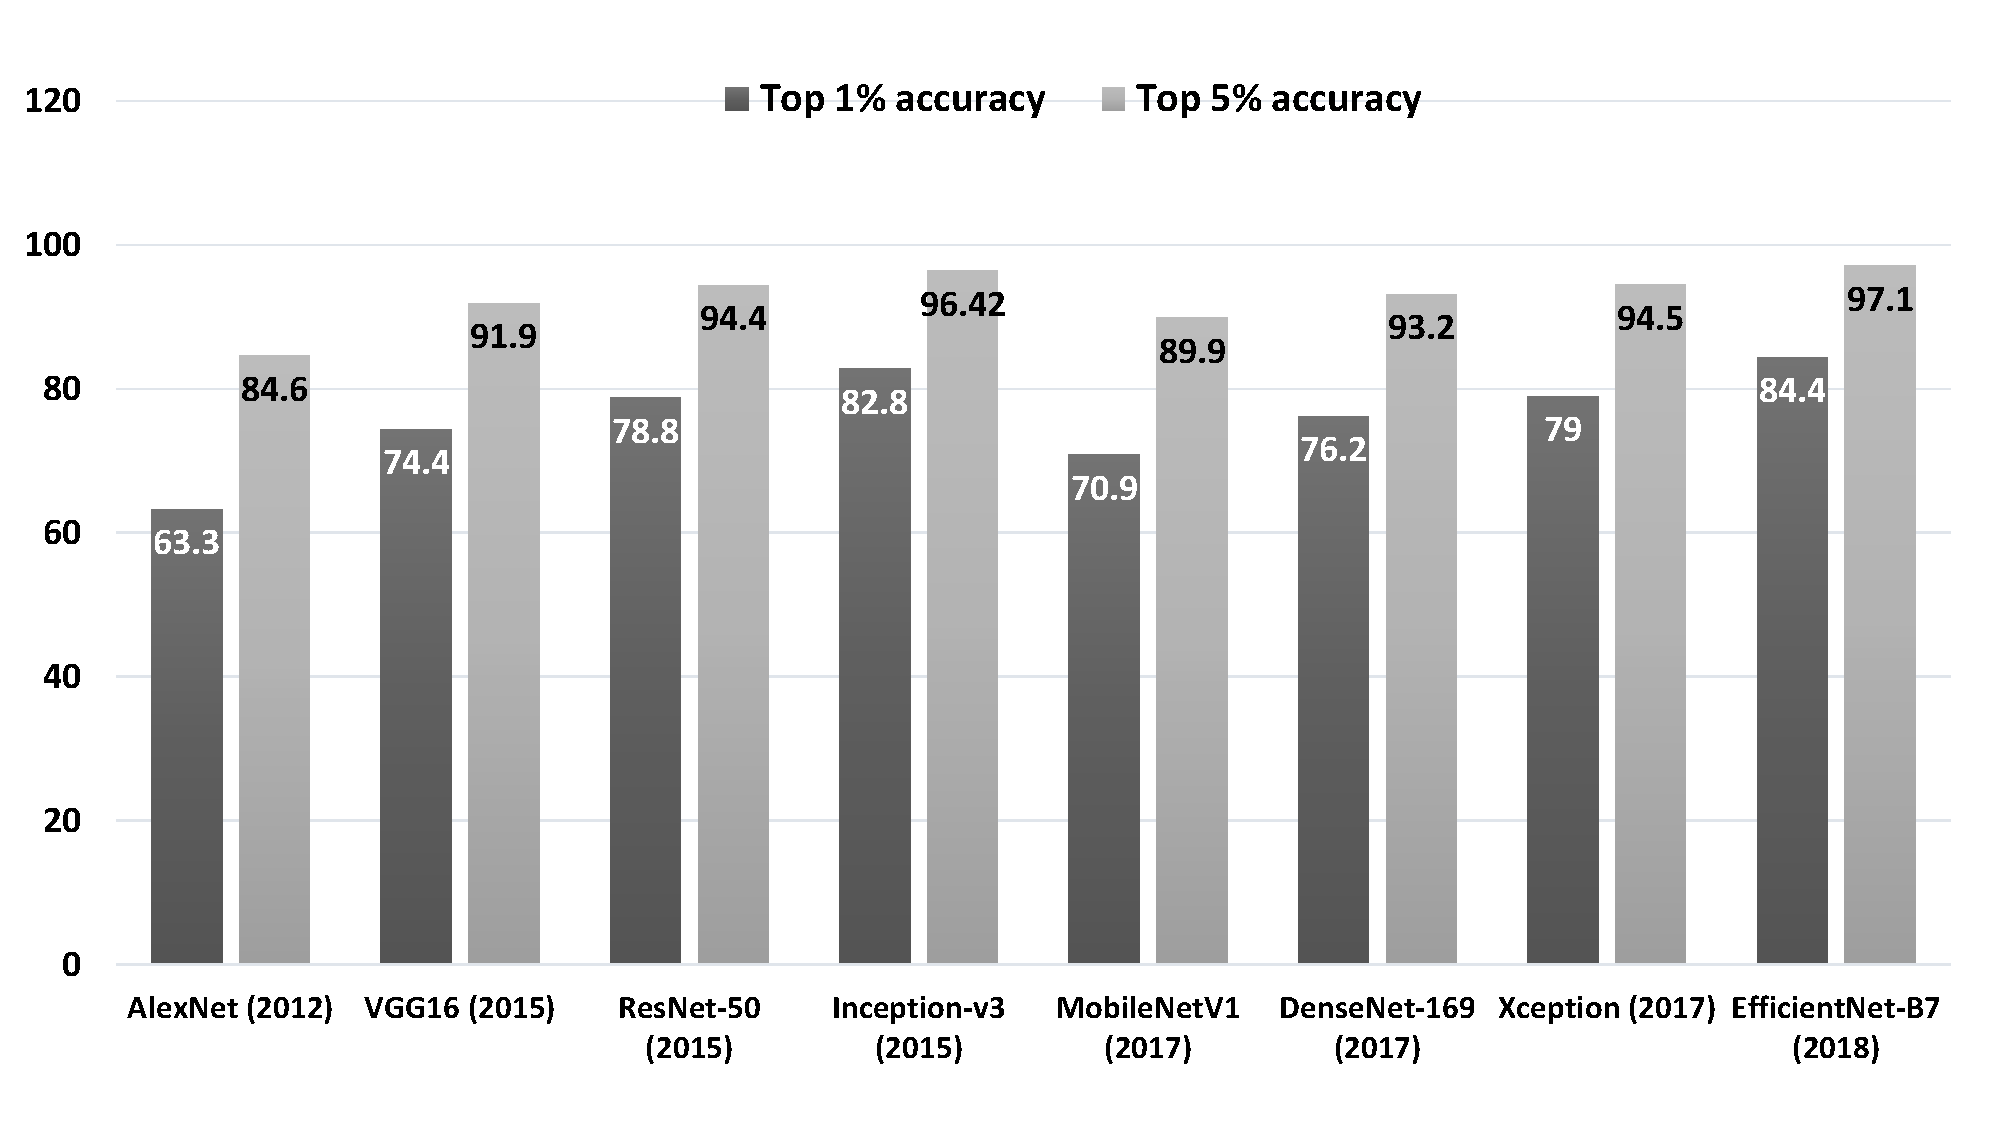
\includegraphics[scale=0.3]{Module 4 (CNN)/pics/accuracy.pdf}

{Comparison of top 1\% and top 5\% accuracy of different CNNs.}
\end{center}


    
\end{frame}
\begin{frame}{Comparisons}
\begin{center}
\vspace{-0.7cm}
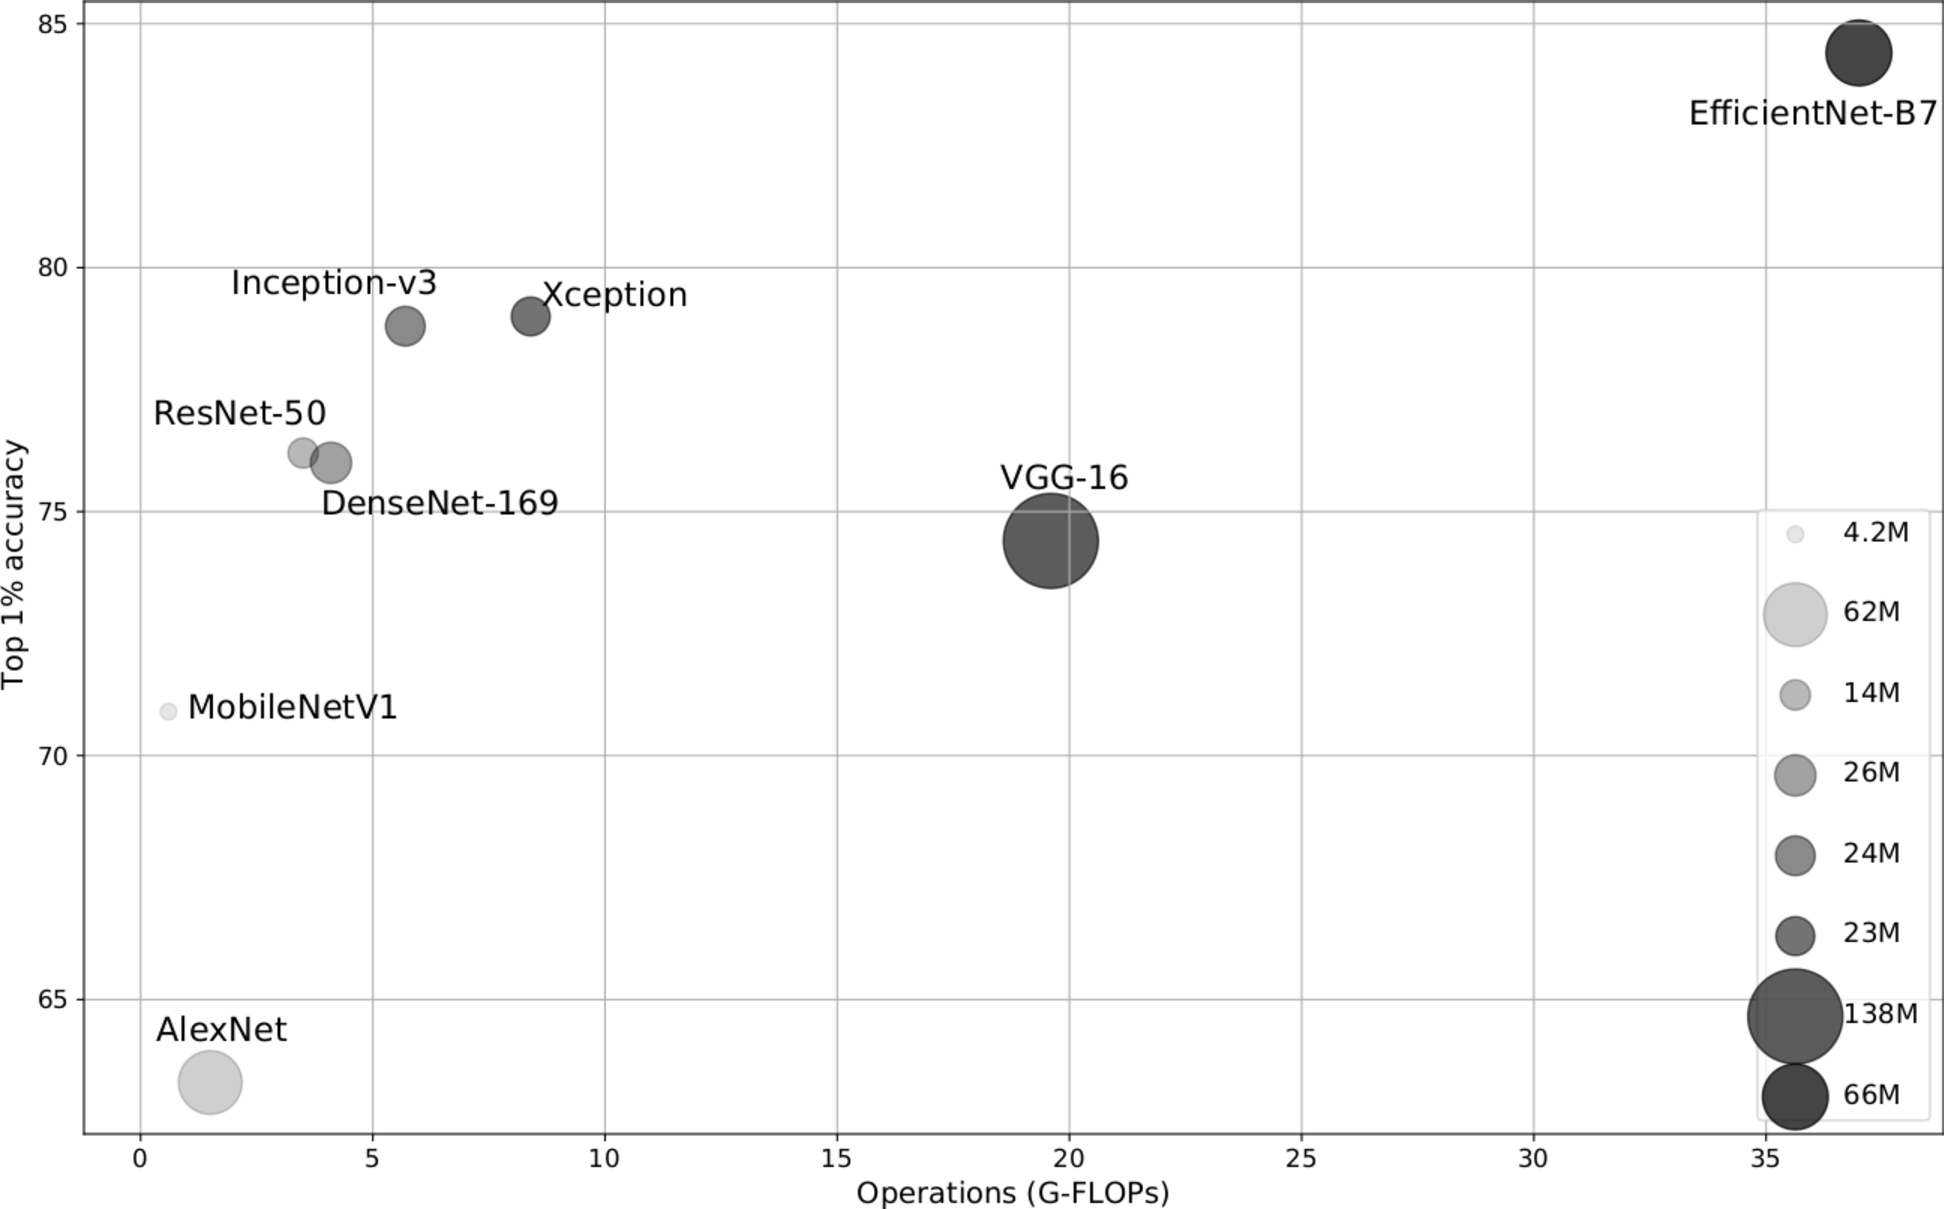
\includegraphics[scale=0.3]{Module 4 (CNN)/pics/gflop_acc_param_CNNnets.pdf}
\end{center}
Comparison of top 1\% accuracy, Number of parameters and operations (G-FLOPS) of different CNN architectures for image classification.

    
\end{frame}

\end{document}
